\section{Implementation}

The algorithm was created in python 3 using scikit-learn coding guidelines and API conventions. The Classes will be defined as shown in \ref{uml:rpkm} UML diagram.

\begin{center}
    \begin{tikzpicture}
    \begin{umlpackage}{rpkm}
        \umlclass[]{Subset}{
            indexes : np.ndarray $(N, F$)\\ 
            max : np.ndarray $(F, )$ \\
            min : np.ndarray $(F, )$ \\
            thresholds: np.ndarray $(F, )$ \\
        }{
            representative : np.ndarray $(F, )$ \\
            \_\_len\_\_: int \\
        }
        \umlclass[y=-5, template=BaseEstimator ClusterMixin ClassifierMixin]{RPKM}{
            n\_clusters : int \\ 
            max\_iter : int \\
            distance\_threshold: float \\
            centroids: None or np.ndarray $(n_{clusters}, F)$ \\
            distance\_computations: int \\
            instance\_ratio: float \\
        }{
            fit: RPKM \\
            predict: np.array $(n_{predict},)$ \\
            fit\_predict: np.array $(n_{predict},)$ \\
        }
    \end{umlpackage}
    \label{uml:rpkm}
    \end{tikzpicture}
\end{center}

Only the public methods are specified in the diagram. $N$ in the diagram represents the number of instances in a subset. The $F$ value indicates the number of features in the dataset. $n_{predict}$ represents the number of instances to be predicted in the inference dataset.

\section{Subset}

Subset would be a struct in other programming languages but in python it is defined as a class. The class contains:

\begin{enumerate}
    \item \textbf{The indexes of the original data in this subset.} This is done in order to store pointers to a data structure instead of cloning the memory on the numpy arrays, as for massive datasets this can lead to memory issues. 
    \item \textbf{The minimum and maximum range} per each of the dimensions on the dataset and the thresholds used to build the next partition from this subset. 
    \item The threshold $t$ is defined as the value that divides the range in to equal size subspaces for each dimension $\overrightarrow{t} = \frac{\overrightarrow{max} + \overrightarrow{min}}{2}$. 
    \item A method to compute the \textbf{cardinality}. In this case python's \_\_len\_\_ method is used to return the length of the index array.
    \item A method to compute the \textbf{representative} for the cluster. As mentioned before, this is computed as the mean of the instances in the subset. The \textit{np.mean} function was used to perform the operation effectively.
\end{enumerate}

The Subset class has been created to follow an obejct oriented approach to the data structures.

\section{RPKM}

The RPKM algorithm was implemented in another class which inherits from \textit{sklearn's BaseEstimator , ClassifierMixin and ClusterMixin} classes. The \textit{BaseEstimator} is the main base class that all sklearn estimators inherit from. it provides parameter setters and getters for the class as well as a string representation of the class as well as some utility methods.

\begin{enumerate}
    \item \textbf{set\_params(**params)}: Set the parameters of this estimator.
    \item \textbf{get\_params()}: Get parameters for this estimator.
    \item \textbf{\_\_repr\_\_()}: String representation of the estimator
    \item \textbf{\_validate\_data(X)}: Validate input data and set or check the \textit{n\_features\_in\_} attribute, also of BaseEstimator.
\end{enumerate}

The ClassifierMixin provides methods for all classifiers in the scikit-learn package. It implements the \textbf{score(X, y)} method to predict the labels for the data X and then compute the accuracy wrt y.

The ClusterMixin provides methods for all clustering methods in the scikit-learn package. It implements the \textbf{fit\_predict(X, y=None)} method to fit the estimator and return the labels for the training data.

In the following subsections we will explain parts of RPKM's fit method that implements the method described by the authors to recursively partition the feature space into hypercubes.

\subsection{fit}

The fit method is the responsible of computing the partition and it's subsets for each RPKM iteration and apply a WL algorithm in every step. The algorithm in pseudocode is presented in \ref{algo:fit}.


\begin{algorithm}[H]
    \SetAlgoLined
    \KwIn{Dataset D, number of clusters K, maximum number of iterations m}
    \KwOut{Self}
    reset centers\;
    Initialize $P_0 = \{D\}$\;
    i := 0\;
    \While{$i < m$}{
        create next partition (\_create\_partition)\;
        compute $R$ and $cardinality$ of the subsets (\_compute\_partition\_meta)\;
        \uIf{$|P_i| < K$}{
            there are not enough partitions to initialize clusters.\;
            \textbf{continue}\;
        }
        \uElseIf{centroids not initialized}{
            choose K random representatives as cluster centers\;
        }
        \uElseIf{$|P_i| >= K$}{
            there are as many subsets as samples, no point in continuing.\;
            \textbf{break}\;
        }
        update clusters with WL (\_cluster)\;
        i += 1\;
    }
    \KwRet{Self}
    \label{algo:fit}
    \caption{RPKM Fit}
\end{algorithm}

The fit algorithm contains the main loop for the RPKM algorithm. One notable difference between the proposal of the authors and the implementation presented in this work is the change in the partition creation. The authors propose the creation of the partitions outside of the loop, creating always $m$ partitions of the dataset. The method proposed here is to generate only the partitions that we require by integrating the creation of the partitions in the while loop. By doing this we are only computing the partitions that are required for the run (in case we reach the number of instances earlier than the iteration $m$).

The fit method calls internally to 3 methods: \textbf{\_create\_partition(X, partition)}, \\ \textbf{\_compute\_partition\_meta(X, partition)}, and \textbf{\_cluster(R, cardinality)}. Each of the methods will be now explained.

\subsection{\_create\_partition}
The create partition method is the one reponsible of, given a list of sets that constitute a partition, perform a binary partition on each subset and create a list containing the new subsets. For the sake of brevity, the binary partition methodology will be explained in this section.

The binary partition method segments the data given as an input that constutes a subset $S$ of the previous iteration's partition $P_{i-1}$. The subsets are created by taking the input data and a set of thresholds defined as the values that partition a dimension in two equally sized hypercubes. This operation is done for each of the dimensions in the dataset. The operation is performed by the following numpy operation: 

\begin{lstlisting}[language=python]
comps = X > subset.thresholds[None, :]
\end{lstlisting}

This operation will generate a numpy matrix with boolean values with shape $(n_{subset}, n_{dim})$ where each row will contain the binary representation of a numerical index assigned to each hypercube. This matrix will be converted to an array of integer indexes containing the assignation of each of the elements to a subset. The conversion from binary to int is performed by the \textit{np.packbits} method.

After the indexes are computed, the subsets initialized using the Subset struct described above, where the min, max and threshold arrays are modified to suit the new subset's instances. The range is modified in the following way:

If the binary representation for the cluster integer value has the value 1 in a dimension position, it means that the comparison performed before was true, so all instances are in the positive half of the spatial partitions. Because of that, the minimum for that dimension is updated to be the threshold value for that dimension. On the other hand, if the value is 0 for that dimension, the max for that dimension is set to be the threshold value for that dimension. Then the threshold values are updated to be the mean between the min and the max arrays. The subsets are then returned for the create partition function to concatenate them all and build the new partition.

\subsection{\_compute\_partition\_meta}

The compute partition meta method is responsible for the generation of the representatives for each subset in the partition as well as the cardinality values for each subset.
This method initializes the R vector to be of shape $(n_{subsets}, n_{features})$ and the cardinality array to be of shape $(n_{subsets}, )$. Once the arrays are initialized it procedes to populate the arrays with the result of the \textbf{representative} function of the Subset class and the length of the Subset class respectively.

\subsection{\_cluster}

The cluster method is in charge of updating the centroids of the RPKM algorithm by fitting a WL algorithm with the representatives as data points and the cardinality of the subsets as the weights. In the implementation, \textit{scikit-learn's KMeans} object was used with the \textit{n\_iter} parameter set to 1 and giving as argument the weights into the fit method. It's also important to note that KMeans supports Lloyd's algorithm as well as Elkan optimization. In order to ensure the usage of Lloyd's algorithm, the \textit{algorithm} parameter must be set to \textit{full}. As initialization for the KMeans algorithm, the centroids of the previous RPKM iteration are passed. After the algorithm is fitted, the cluster centers are extracted by accessing the \textit{cluster\_centers\_} attribute of KMeans.

\section{fit results}

Once the implementation was done, we demonstrate the operation of the algorithm. We will use a 2 dimensional gaussian mixture with 3 gaussian distributions. The RPKM algorithm was performed with the max iterations of $m=6$. On the first figure \ref{fig:partitions2} we represent the creation of the partitions. where the dataset comprised in the range -1, 1 for both dimensions. In the first iteration, the subsets are the 4 quadrants of the subspace, on the next iteration, each quadrant is divided in 4, and so on. We represent each subset with different colors for better interpretability.

\begin{figure}[!ht]
    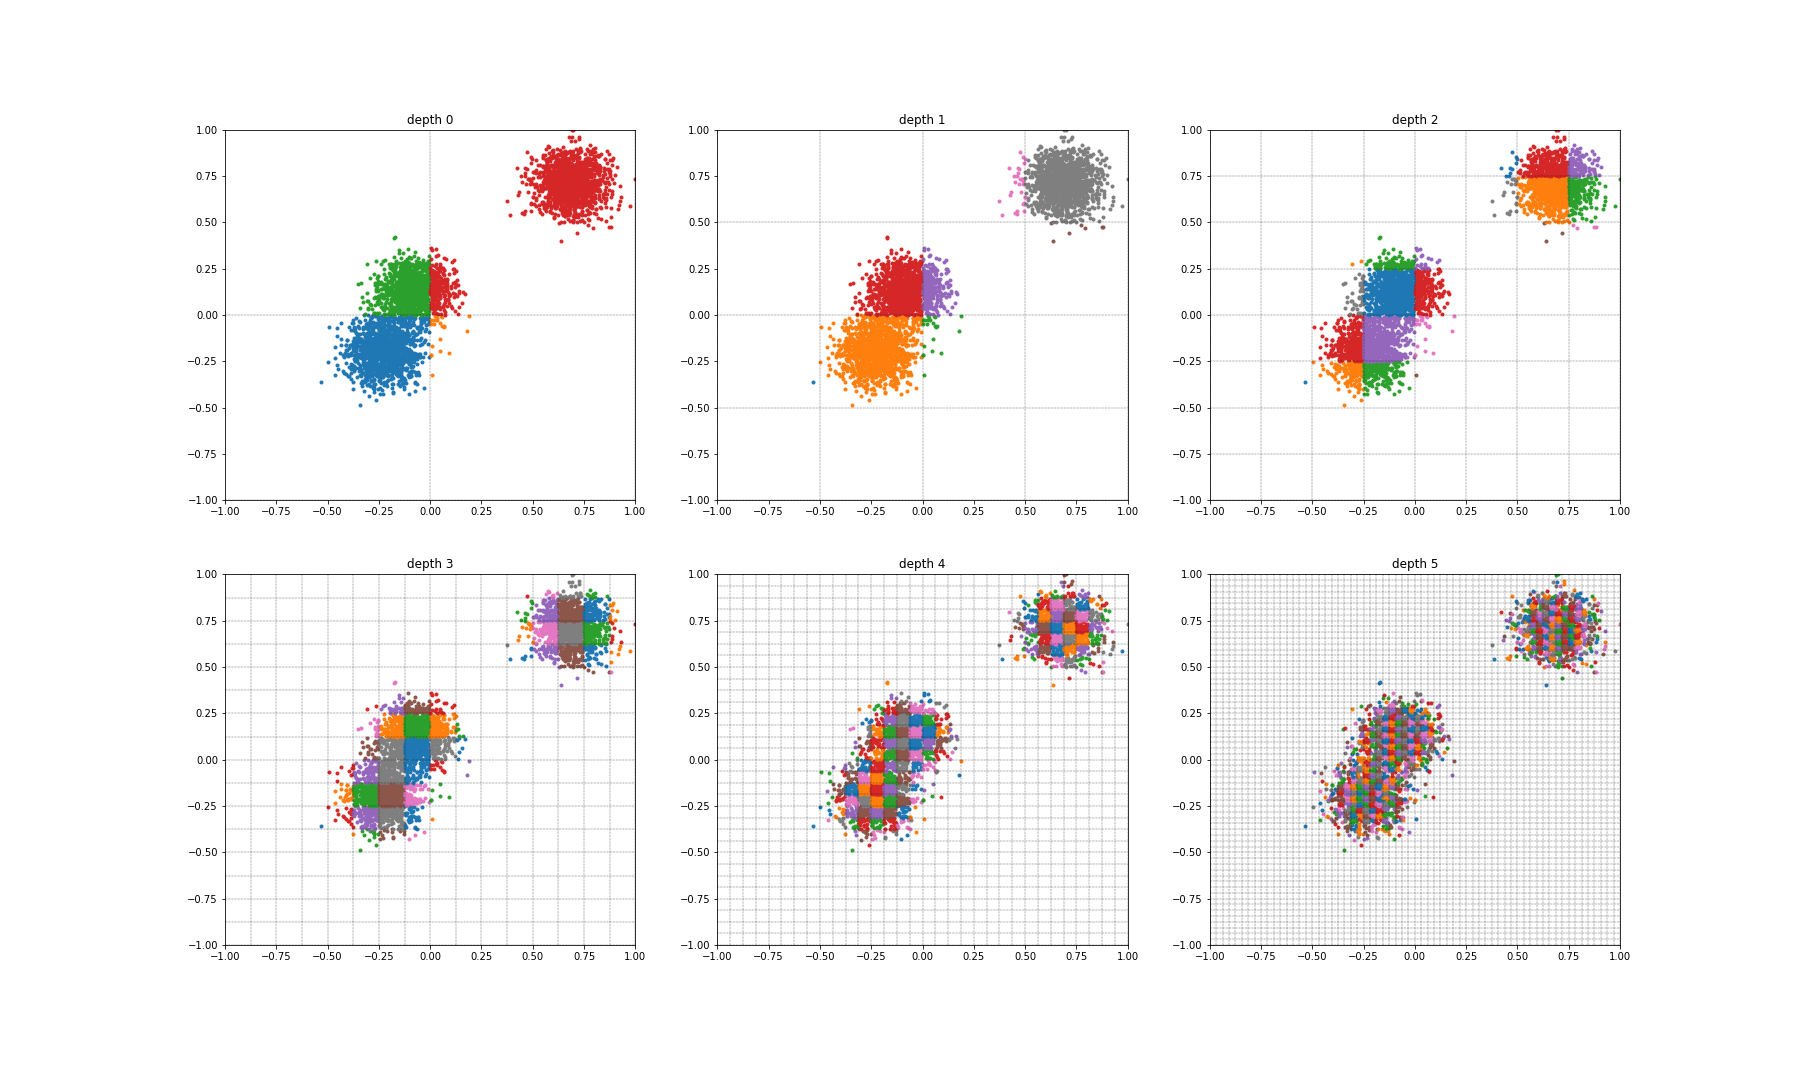
\includegraphics[width=\linewidth]{images/alldepths.png}
    \caption{Partition example for a 2d gaussian mixture}
    \label{fig:partitions2}
\end{figure}

In the next figure \ref{fig:steps} we represent the data in light gray, the representative sampels for each of the subsets in black and the centers with more vivid colors.

\begin{figure}[!ht]
    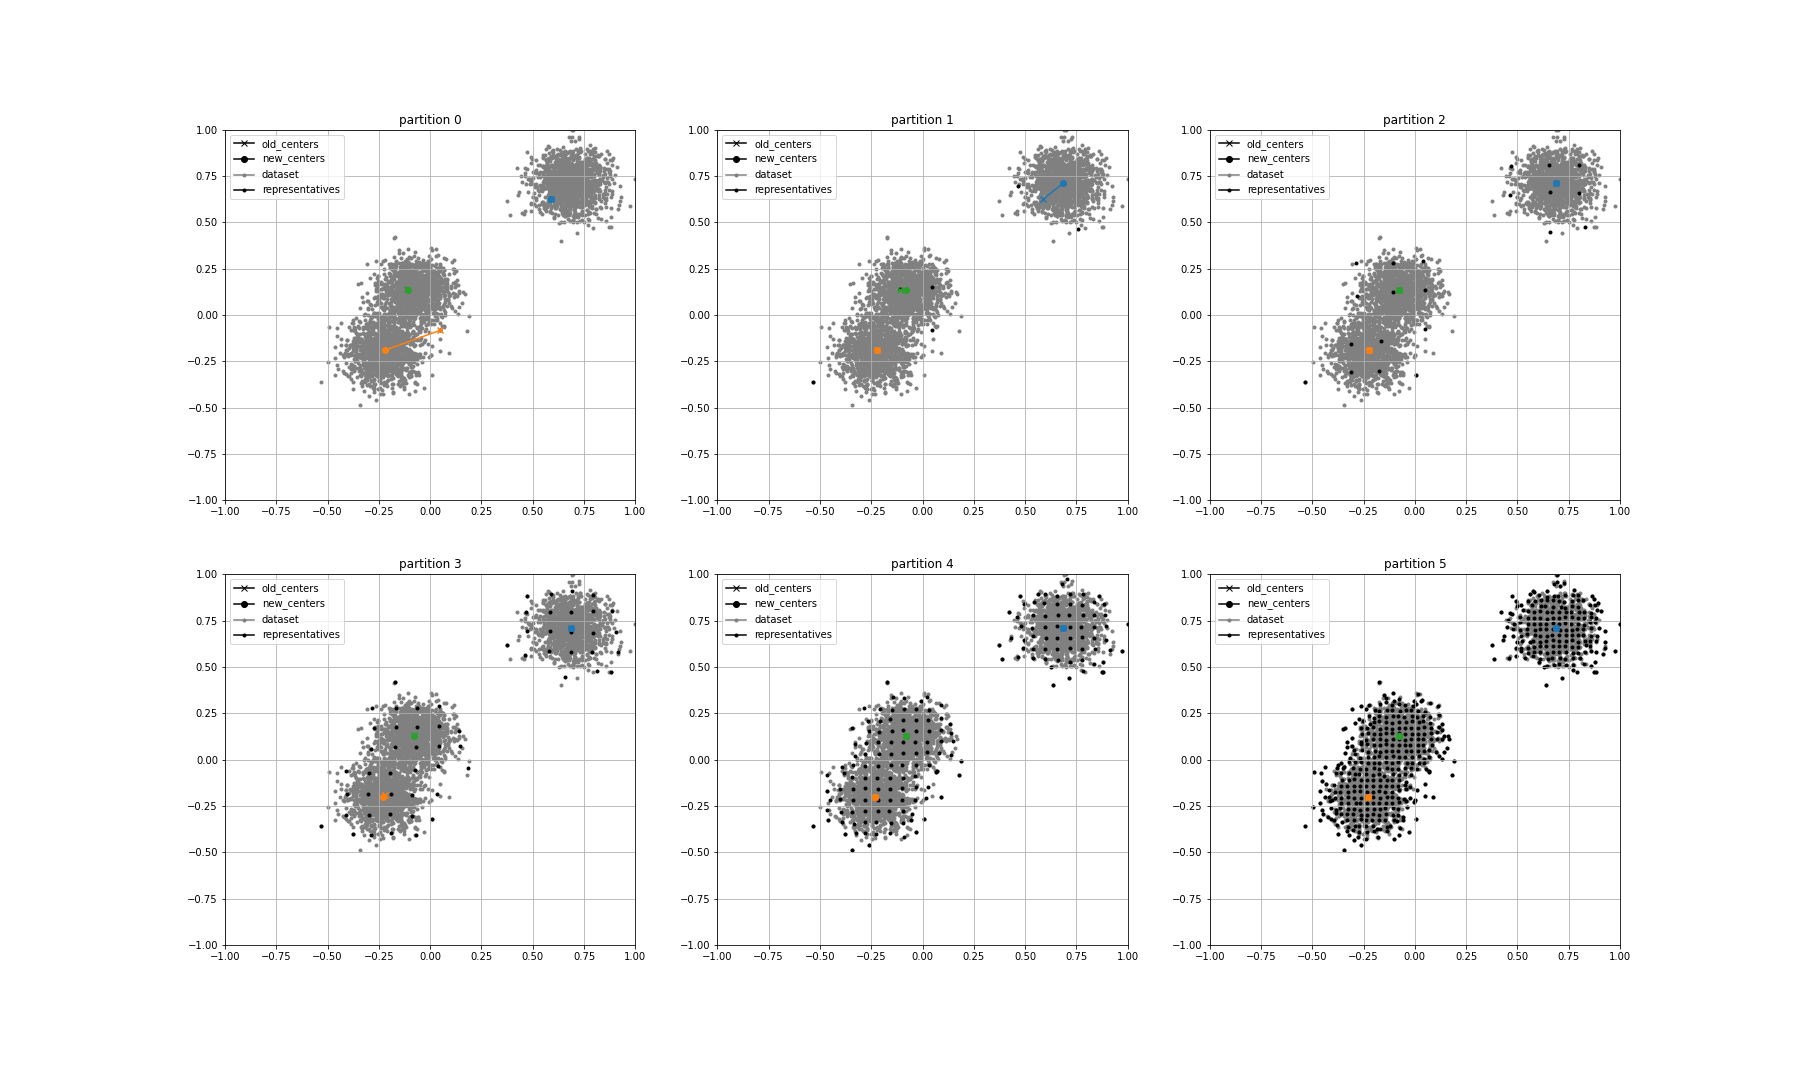
\includegraphics[width=\linewidth]{images/steps.png}
    \caption{Centers and representatives in each iteration}
    \label{fig:steps}
\end{figure}

Finally, the last figure \ref{fig:summary_iteration} represent the evolution of the centers from iteration of iteration. And how the centers approximate more and more the centers of the gaussian distributions.

\begin{figure}[!ht]
    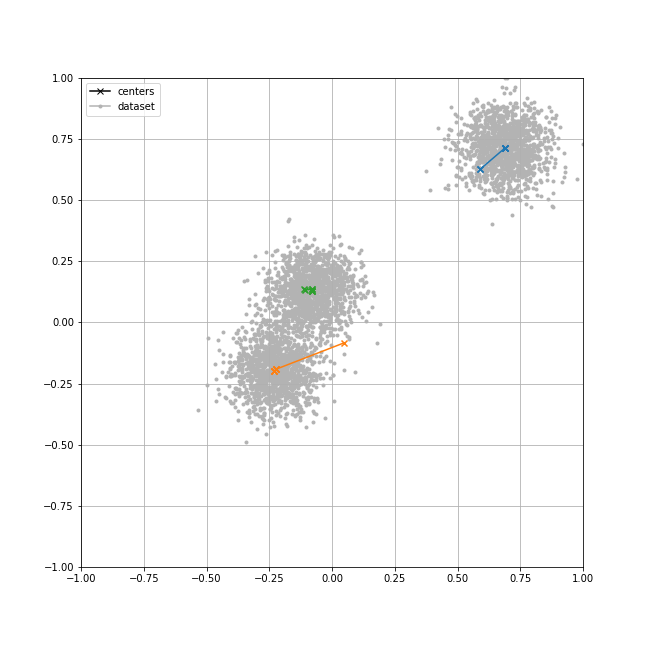
\includegraphics[width=\linewidth]{images/summary_iteration.png}
    \caption{Center evolution}
    \label{fig:summary_iteration}
\end{figure}

\section{Artificial Dataset Generator}

Additionally to the algorithm classes, a helper class able to generate datasets as specified in the paper was required to do the experiments with the artificial datasets. In the paper they specify that they create gaussian mixture datasets ensuring an overlap of less than 5\%. A class was defined as the \textit{Artificial Dataset Generator}. The class is defined in \textit{./src/artificial\_dataset\_generator.py} and each time a new dataset is requested, a random set of centers in the feature space is created. Then the closest centers are detected and the overlap between gaussians is computed. Starting from an std value of 0.1, the value is modified until the maximum overlap between any two gaussians in the dataset is 0.05 and then the dataset is created with sklearn's \textit{datasets.make\_blobs}.
